% Options for packages loaded elsewhere
% Options for packages loaded elsewhere
\PassOptionsToPackage{unicode}{hyperref}
\PassOptionsToPackage{hyphens}{url}
\PassOptionsToPackage{dvipsnames,svgnames,x11names}{xcolor}
%
\documentclass[
]{article}
\usepackage{xcolor}
\usepackage{amsmath,amssymb}
\setcounter{secnumdepth}{5}
\usepackage{iftex}
\ifPDFTeX
  \usepackage[T1]{fontenc}
  \usepackage[utf8]{inputenc}
  \usepackage{textcomp} % provide euro and other symbols
\else % if luatex or xetex
  \usepackage{unicode-math} % this also loads fontspec
  \defaultfontfeatures{Scale=MatchLowercase}
  \defaultfontfeatures[\rmfamily]{Ligatures=TeX,Scale=1}
\fi
\usepackage{lmodern}
\ifPDFTeX\else
  % xetex/luatex font selection
\fi
% Use upquote if available, for straight quotes in verbatim environments
\IfFileExists{upquote.sty}{\usepackage{upquote}}{}
\IfFileExists{microtype.sty}{% use microtype if available
  \usepackage[]{microtype}
  \UseMicrotypeSet[protrusion]{basicmath} % disable protrusion for tt fonts
}{}
\makeatletter
\@ifundefined{KOMAClassName}{% if non-KOMA class
  \IfFileExists{parskip.sty}{%
    \usepackage{parskip}
  }{% else
    \setlength{\parindent}{0pt}
    \setlength{\parskip}{6pt plus 2pt minus 1pt}}
}{% if KOMA class
  \KOMAoptions{parskip=half}}
\makeatother
% Make \paragraph and \subparagraph free-standing
\makeatletter
\ifx\paragraph\undefined\else
  \let\oldparagraph\paragraph
  \renewcommand{\paragraph}{
    \@ifstar
      \xxxParagraphStar
      \xxxParagraphNoStar
  }
  \newcommand{\xxxParagraphStar}[1]{\oldparagraph*{#1}\mbox{}}
  \newcommand{\xxxParagraphNoStar}[1]{\oldparagraph{#1}\mbox{}}
\fi
\ifx\subparagraph\undefined\else
  \let\oldsubparagraph\subparagraph
  \renewcommand{\subparagraph}{
    \@ifstar
      \xxxSubParagraphStar
      \xxxSubParagraphNoStar
  }
  \newcommand{\xxxSubParagraphStar}[1]{\oldsubparagraph*{#1}\mbox{}}
  \newcommand{\xxxSubParagraphNoStar}[1]{\oldsubparagraph{#1}\mbox{}}
\fi
\makeatother

\usepackage{color}
\usepackage{fancyvrb}
\newcommand{\VerbBar}{|}
\newcommand{\VERB}{\Verb[commandchars=\\\{\}]}
\DefineVerbatimEnvironment{Highlighting}{Verbatim}{commandchars=\\\{\}}
% Add ',fontsize=\small' for more characters per line
\usepackage{framed}
\definecolor{shadecolor}{RGB}{241,243,245}
\newenvironment{Shaded}{\begin{snugshade}}{\end{snugshade}}
\newcommand{\AlertTok}[1]{\textcolor[rgb]{0.68,0.00,0.00}{#1}}
\newcommand{\AnnotationTok}[1]{\textcolor[rgb]{0.37,0.37,0.37}{#1}}
\newcommand{\AttributeTok}[1]{\textcolor[rgb]{0.40,0.45,0.13}{#1}}
\newcommand{\BaseNTok}[1]{\textcolor[rgb]{0.68,0.00,0.00}{#1}}
\newcommand{\BuiltInTok}[1]{\textcolor[rgb]{0.00,0.23,0.31}{#1}}
\newcommand{\CharTok}[1]{\textcolor[rgb]{0.13,0.47,0.30}{#1}}
\newcommand{\CommentTok}[1]{\textcolor[rgb]{0.37,0.37,0.37}{#1}}
\newcommand{\CommentVarTok}[1]{\textcolor[rgb]{0.37,0.37,0.37}{\textit{#1}}}
\newcommand{\ConstantTok}[1]{\textcolor[rgb]{0.56,0.35,0.01}{#1}}
\newcommand{\ControlFlowTok}[1]{\textcolor[rgb]{0.00,0.23,0.31}{\textbf{#1}}}
\newcommand{\DataTypeTok}[1]{\textcolor[rgb]{0.68,0.00,0.00}{#1}}
\newcommand{\DecValTok}[1]{\textcolor[rgb]{0.68,0.00,0.00}{#1}}
\newcommand{\DocumentationTok}[1]{\textcolor[rgb]{0.37,0.37,0.37}{\textit{#1}}}
\newcommand{\ErrorTok}[1]{\textcolor[rgb]{0.68,0.00,0.00}{#1}}
\newcommand{\ExtensionTok}[1]{\textcolor[rgb]{0.00,0.23,0.31}{#1}}
\newcommand{\FloatTok}[1]{\textcolor[rgb]{0.68,0.00,0.00}{#1}}
\newcommand{\FunctionTok}[1]{\textcolor[rgb]{0.28,0.35,0.67}{#1}}
\newcommand{\ImportTok}[1]{\textcolor[rgb]{0.00,0.46,0.62}{#1}}
\newcommand{\InformationTok}[1]{\textcolor[rgb]{0.37,0.37,0.37}{#1}}
\newcommand{\KeywordTok}[1]{\textcolor[rgb]{0.00,0.23,0.31}{\textbf{#1}}}
\newcommand{\NormalTok}[1]{\textcolor[rgb]{0.00,0.23,0.31}{#1}}
\newcommand{\OperatorTok}[1]{\textcolor[rgb]{0.37,0.37,0.37}{#1}}
\newcommand{\OtherTok}[1]{\textcolor[rgb]{0.00,0.23,0.31}{#1}}
\newcommand{\PreprocessorTok}[1]{\textcolor[rgb]{0.68,0.00,0.00}{#1}}
\newcommand{\RegionMarkerTok}[1]{\textcolor[rgb]{0.00,0.23,0.31}{#1}}
\newcommand{\SpecialCharTok}[1]{\textcolor[rgb]{0.37,0.37,0.37}{#1}}
\newcommand{\SpecialStringTok}[1]{\textcolor[rgb]{0.13,0.47,0.30}{#1}}
\newcommand{\StringTok}[1]{\textcolor[rgb]{0.13,0.47,0.30}{#1}}
\newcommand{\VariableTok}[1]{\textcolor[rgb]{0.07,0.07,0.07}{#1}}
\newcommand{\VerbatimStringTok}[1]{\textcolor[rgb]{0.13,0.47,0.30}{#1}}
\newcommand{\WarningTok}[1]{\textcolor[rgb]{0.37,0.37,0.37}{\textit{#1}}}

\usepackage{longtable,booktabs,array}
\usepackage{calc} % for calculating minipage widths
% Correct order of tables after \paragraph or \subparagraph
\usepackage{etoolbox}
\makeatletter
\patchcmd\longtable{\par}{\if@noskipsec\mbox{}\fi\par}{}{}
\makeatother
% Allow footnotes in longtable head/foot
\IfFileExists{footnotehyper.sty}{\usepackage{footnotehyper}}{\usepackage{footnote}}
\makesavenoteenv{longtable}
\usepackage{graphicx}
\makeatletter
\newsavebox\pandoc@box
\newcommand*\pandocbounded[1]{% scales image to fit in text height/width
  \sbox\pandoc@box{#1}%
  \Gscale@div\@tempa{\textheight}{\dimexpr\ht\pandoc@box+\dp\pandoc@box\relax}%
  \Gscale@div\@tempb{\linewidth}{\wd\pandoc@box}%
  \ifdim\@tempb\p@<\@tempa\p@\let\@tempa\@tempb\fi% select the smaller of both
  \ifdim\@tempa\p@<\p@\scalebox{\@tempa}{\usebox\pandoc@box}%
  \else\usebox{\pandoc@box}%
  \fi%
}
% Set default figure placement to htbp
\def\fps@figure{htbp}
\makeatother





\setlength{\emergencystretch}{3em} % prevent overfull lines

\providecommand{\tightlist}{%
  \setlength{\itemsep}{0pt}\setlength{\parskip}{0pt}}



 


\makeatletter
\@ifpackageloaded{caption}{}{\usepackage{caption}}
\AtBeginDocument{%
\ifdefined\contentsname
  \renewcommand*\contentsname{Table of contents}
\else
  \newcommand\contentsname{Table of contents}
\fi
\ifdefined\listfigurename
  \renewcommand*\listfigurename{List of Figures}
\else
  \newcommand\listfigurename{List of Figures}
\fi
\ifdefined\listtablename
  \renewcommand*\listtablename{List of Tables}
\else
  \newcommand\listtablename{List of Tables}
\fi
\ifdefined\figurename
  \renewcommand*\figurename{Figure}
\else
  \newcommand\figurename{Figure}
\fi
\ifdefined\tablename
  \renewcommand*\tablename{Table}
\else
  \newcommand\tablename{Table}
\fi
}
\@ifpackageloaded{float}{}{\usepackage{float}}
\floatstyle{ruled}
\@ifundefined{c@chapter}{\newfloat{codelisting}{h}{lop}}{\newfloat{codelisting}{h}{lop}[chapter]}
\floatname{codelisting}{Listing}
\newcommand*\listoflistings{\listof{codelisting}{List of Listings}}
\makeatother
\makeatletter
\makeatother
\makeatletter
\@ifpackageloaded{caption}{}{\usepackage{caption}}
\@ifpackageloaded{subcaption}{}{\usepackage{subcaption}}
\makeatother
\usepackage{bookmark}
\IfFileExists{xurl.sty}{\usepackage{xurl}}{} % add URL line breaks if available
\urlstyle{same}
\hypersetup{
  pdftitle={House Prices: Advanced Regression Techniques},
  pdfauthor={Wanshu He},
  pdfkeywords={survey research, python, quarto},
  colorlinks=true,
  linkcolor={blue},
  filecolor={Maroon},
  citecolor={Blue},
  urlcolor={Blue},
  pdfcreator={LaTeX via pandoc}}


\title{House Prices: Advanced Regression Techniques}
\author{Wanshu He}
\date{2025-08-08}
\begin{document}
\maketitle
\begin{abstract}
Abstract: This study presents a comprehensive data science project
exploring the \textbf{Ames Housing} dataset from the Kaggle competition
``House Prices -- Advanced Regression Techniques''. The goal is to
predict residential home sale prices using a wide range of explanatory
variables and apply various machine learning techniques. We will perform
exploratory data analysis, clean and preprocess the data, build several
regression models, including basic baselines as well as neural networks
and tree-based models, then compare their performance, and finally make
a prediction file for submission to Kaggle competition. We will also
simulate a SQL database query to demonstrate data manipulation
capabilities.
\end{abstract}

\renewcommand*\contentsname{Table of contents}
{
\hypersetup{linkcolor=}
\setcounter{tocdepth}{3}
\tableofcontents
}

\section{Dataset Overview}\label{dataset-overview}

The dataset contains \textbf{79 explanatory variables} describing
different aspects of residential homes in Ames, Iowa.\\
Key fields include:

\begin{itemize}
\tightlist
\item
  \texttt{SalePrice}: the target variable representing the sale price of
  the house.
\item
  \texttt{MSSubClass}: building class.
\item
  \texttt{MSZoning}: general zoning classification.
\item
  \texttt{LotFrontage}: linear feet of street connected to the property.
\item
  \texttt{OverallQual}: overall material and finish quality.
\item
  \texttt{GrLivArea}: above ground living area (in square feet).
\item
  \ldots{}
\end{itemize}

The training set contains 1,460 observations with 81 columns (including
\texttt{SalePrice}), while the test set contains 1,459 observations with
80 columns (missing \texttt{SalePrice}).

We aim to predict \texttt{SalePrice} for the test set and evaluate
models using Root Mean Squared Error (RMSE) on the log-transformed
prices (as per the competition's metric).

\begin{Shaded}
\begin{Highlighting}[]
\CommentTok{\# Load the training and test datasets}
\NormalTok{train\_df }\OperatorTok{=}\NormalTok{ pd.read\_csv(}\StringTok{\textquotesingle{}train.csv\textquotesingle{}}\NormalTok{)}
\NormalTok{test\_df }\OperatorTok{=}\NormalTok{ pd.read\_csv(}\StringTok{\textquotesingle{}test.csv\textquotesingle{}}\NormalTok{)}

\CommentTok{\# Display the first few rows of the training data and basic info}
\BuiltInTok{print}\NormalTok{(}\StringTok{\textquotesingle{}Training data shape:\textquotesingle{}}\NormalTok{, train\_df.shape)}
\BuiltInTok{print}\NormalTok{(}\StringTok{\textquotesingle{}Test data shape:\textquotesingle{}}\NormalTok{, test\_df.shape)}
\NormalTok{train\_df.head()}
\end{Highlighting}
\end{Shaded}

\begin{verbatim}
Training data shape: (1460, 81)
Test data shape: (1459, 80)
\end{verbatim}

\begin{longtable}[]{@{}llllllllllllllllllllll@{}}
\toprule\noalign{}
& Id & MSSubClass & MSZoning & LotFrontage & LotArea & Street & Alley &
LotShape & LandContour & Utilities & ... & PoolArea & PoolQC & Fence &
MiscFeature & MiscVal & MoSold & YrSold & SaleType & SaleCondition &
SalePrice \\
\midrule\noalign{}
\endhead
\bottomrule\noalign{}
\endlastfoot
0 & 1 & 60 & RL & 65.0 & 8450 & Pave & NaN & Reg & Lvl & AllPub & ... &
0 & NaN & NaN & NaN & 0 & 2 & 2008 & WD & Normal & 208500 \\
1 & 2 & 20 & RL & 80.0 & 9600 & Pave & NaN & Reg & Lvl & AllPub & ... &
0 & NaN & NaN & NaN & 0 & 5 & 2007 & WD & Normal & 181500 \\
2 & 3 & 60 & RL & 68.0 & 11250 & Pave & NaN & IR1 & Lvl & AllPub & ... &
0 & NaN & NaN & NaN & 0 & 9 & 2008 & WD & Normal & 223500 \\
3 & 4 & 70 & RL & 60.0 & 9550 & Pave & NaN & IR1 & Lvl & AllPub & ... &
0 & NaN & NaN & NaN & 0 & 2 & 2006 & WD & Abnorml & 140000 \\
4 & 5 & 60 & RL & 84.0 & 14260 & Pave & NaN & IR1 & Lvl & AllPub & ... &
0 & NaN & NaN & NaN & 0 & 12 & 2008 & WD & Normal & 250000 \\
\end{longtable}

\section{Exploratory Data Analysis}\label{exploratory-data-analysis}

Before building models, we explore the distribution of the target
variable and some important features.\\
A look at the sale price distribution reveals skewness, which suggests a
log transformation will be beneficial for regression models.

\begin{Shaded}
\begin{Highlighting}[]
\CommentTok{\# Plot the distribution of the target variable SalePrice}
\NormalTok{plt.figure()}
\NormalTok{plt.hist(train\_df[}\StringTok{\textquotesingle{}SalePrice\textquotesingle{}}\NormalTok{], bins}\OperatorTok{=}\DecValTok{30}\NormalTok{)}
\NormalTok{plt.title(}\StringTok{\textquotesingle{}Distribution of SalePrice\textquotesingle{}}\NormalTok{)}
\NormalTok{plt.xlabel(}\StringTok{\textquotesingle{}SalePrice\textquotesingle{}}\NormalTok{)}
\NormalTok{plt.ylabel(}\StringTok{\textquotesingle{}Frequency\textquotesingle{}}\NormalTok{)}
\NormalTok{plt.show()}

\CommentTok{\# Log{-}transformed SalePrice distribution}
\NormalTok{plt.figure()}
\NormalTok{plt.hist(np.log1p(train\_df[}\StringTok{\textquotesingle{}SalePrice\textquotesingle{}}\NormalTok{]), bins}\OperatorTok{=}\DecValTok{30}\NormalTok{)}
\NormalTok{plt.title(}\StringTok{\textquotesingle{}Distribution of log1p(SalePrice)\textquotesingle{}}\NormalTok{)}
\NormalTok{plt.xlabel(}\StringTok{\textquotesingle{}log1p(SalePrice)\textquotesingle{}}\NormalTok{)}
\NormalTok{plt.ylabel(}\StringTok{\textquotesingle{}Frequency\textquotesingle{}}\NormalTok{)}
\NormalTok{plt.show()}
\end{Highlighting}
\end{Shaded}

\pandocbounded{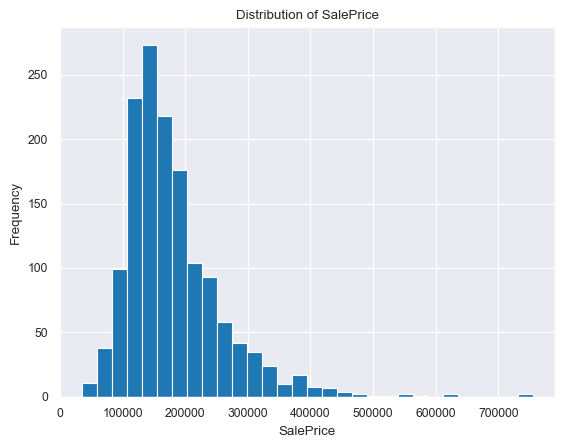
\includegraphics[keepaspectratio]{house_prices_project_files/figure-pdf/cell-4-output-1.png}}

\pandocbounded{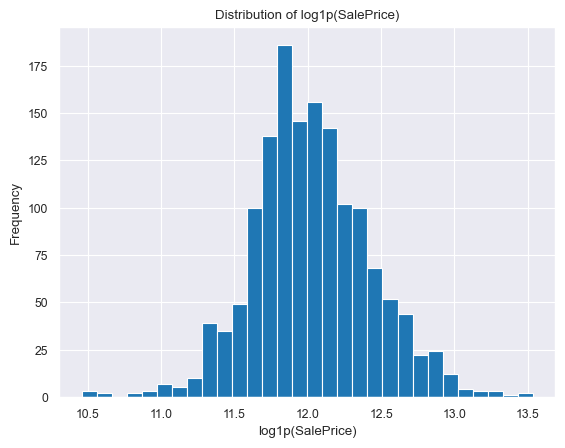
\includegraphics[keepaspectratio]{house_prices_project_files/figure-pdf/cell-4-output-2.png}}

\subsection{SalePrice vs.~Overall
Quality}\label{saleprice-vs.-overall-quality}

House quality (\texttt{OverallQual}) is one of the most influential
features.\\
Below we display a boxplot and a violin plot of \texttt{SalePrice} by
\texttt{OverallQual} to visualize how sale prices vary across quality
levels.

\begin{Shaded}
\begin{Highlighting}[]
\CommentTok{\# Create boxplot of SalePrice by OverallQual}
\NormalTok{plt.figure()}
\CommentTok{\# Prepare data groups for each quality level}
\NormalTok{qualities }\OperatorTok{=} \BuiltInTok{sorted}\NormalTok{(train\_df[}\StringTok{\textquotesingle{}OverallQual\textquotesingle{}}\NormalTok{].unique())}
\NormalTok{boxes }\OperatorTok{=}\NormalTok{ [train\_df[train\_df[}\StringTok{\textquotesingle{}OverallQual\textquotesingle{}}\NormalTok{] }\OperatorTok{==}\NormalTok{ q][}\StringTok{\textquotesingle{}SalePrice\textquotesingle{}}\NormalTok{] }\ControlFlowTok{for}\NormalTok{ q }\KeywordTok{in}\NormalTok{ qualities]}
\NormalTok{plt.boxplot(boxes, labels}\OperatorTok{=}\NormalTok{qualities)}
\NormalTok{plt.title(}\StringTok{\textquotesingle{}SalePrice by OverallQual (Boxplot)\textquotesingle{}}\NormalTok{)}
\NormalTok{plt.xlabel(}\StringTok{\textquotesingle{}Overall Quality\textquotesingle{}}\NormalTok{)}
\NormalTok{plt.ylabel(}\StringTok{\textquotesingle{}SalePrice\textquotesingle{}}\NormalTok{)}
\NormalTok{plt.show()}

\CommentTok{\# Violin plot use sns on boxes}
\ImportTok{import}\NormalTok{ seaborn }\ImportTok{as}\NormalTok{ sns}
\NormalTok{plt.figure()}
\NormalTok{sns.violinplot(x}\OperatorTok{=}\StringTok{\textquotesingle{}OverallQual\textquotesingle{}}\NormalTok{, y}\OperatorTok{=}\StringTok{\textquotesingle{}SalePrice\textquotesingle{}}\NormalTok{, data}\OperatorTok{=}\NormalTok{train\_df)}
\NormalTok{plt.title(}\StringTok{\textquotesingle{}SalePrice by OverallQual (Violin Plot)\textquotesingle{}}\NormalTok{)}
\NormalTok{plt.xlabel(}\StringTok{\textquotesingle{}Overall Quality\textquotesingle{}}\NormalTok{)}
\NormalTok{plt.ylabel(}\StringTok{\textquotesingle{}SalePrice\textquotesingle{}}\NormalTok{)}
\NormalTok{plt.xticks(qualities)}
\NormalTok{plt.show()}
\end{Highlighting}
\end{Shaded}

\pandocbounded{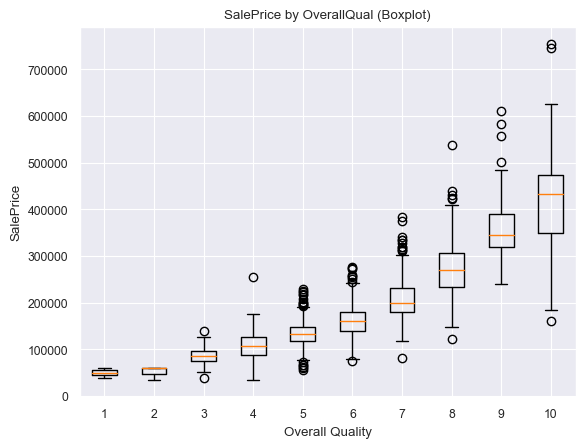
\includegraphics[keepaspectratio]{house_prices_project_files/figure-pdf/cell-5-output-1.png}}

\pandocbounded{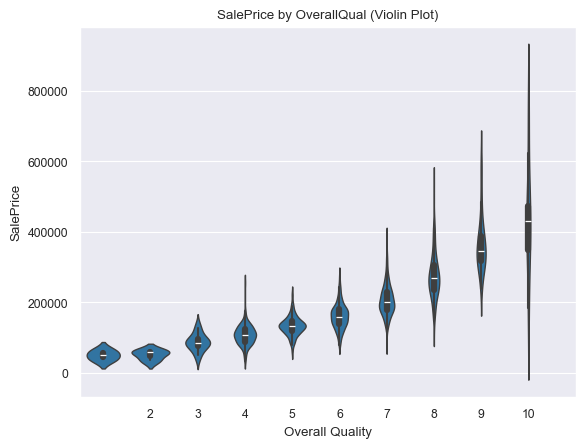
\includegraphics[keepaspectratio]{house_prices_project_files/figure-pdf/cell-5-output-2.png}}

\subsection{Living Area vs.~SalePrice}\label{living-area-vs.-saleprice}

A scatter plot helps illustrate the relationship between the
above-ground living area (\texttt{GrLivArea}) and the sale price.\\
We expect larger homes to sell for higher prices, albeit with some
variability.

\begin{Shaded}
\begin{Highlighting}[]

\CommentTok{\# Scatter plot of GrLivArea vs SalePrice}
\NormalTok{plt.figure()}
\NormalTok{plt.scatter(train\_df[}\StringTok{\textquotesingle{}GrLivArea\textquotesingle{}}\NormalTok{], train\_df[}\StringTok{\textquotesingle{}SalePrice\textquotesingle{}}\NormalTok{])}
\NormalTok{plt.title(}\StringTok{\textquotesingle{}GrLivArea vs SalePrice\textquotesingle{}}\NormalTok{)}
\NormalTok{plt.xlabel(}\StringTok{\textquotesingle{}GrLivArea (sq ft)\textquotesingle{}}\NormalTok{)}
\NormalTok{plt.ylabel(}\StringTok{\textquotesingle{}SalePrice\textquotesingle{}}\NormalTok{)}
\NormalTok{plt.show()}

\CommentTok{\# Scatter plot of GrLivArea vs log1p(SalePrice)}
\NormalTok{plt.figure()}
\NormalTok{plt.scatter(train\_df[}\StringTok{\textquotesingle{}GrLivArea\textquotesingle{}}\NormalTok{], np.log1p(train\_df[}\StringTok{\textquotesingle{}SalePrice\textquotesingle{}}\NormalTok{]))}
\NormalTok{plt.title(}\StringTok{\textquotesingle{}GrLivArea vs log1p(SalePrice)\textquotesingle{}}\NormalTok{)}
\NormalTok{plt.xlabel(}\StringTok{\textquotesingle{}GrLivArea (sq ft)\textquotesingle{}}\NormalTok{)}
\NormalTok{plt.ylabel(}\StringTok{\textquotesingle{}log1p(SalePrice)\textquotesingle{}}\NormalTok{)}
\NormalTok{plt.show()}
\end{Highlighting}
\end{Shaded}

\pandocbounded{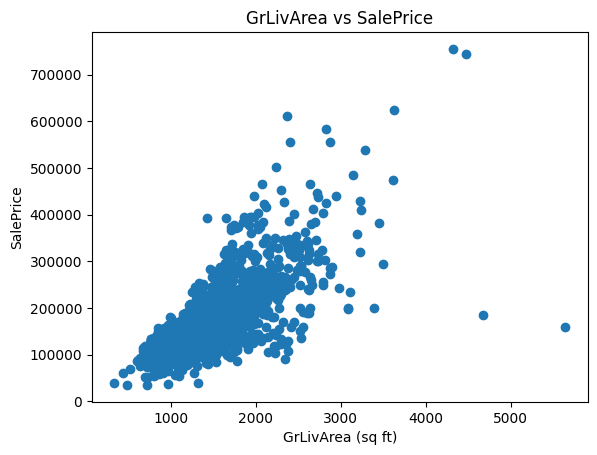
\includegraphics[keepaspectratio]{house_prices_project_files/figure-pdf/cell-6-output-1.png}}

\pandocbounded{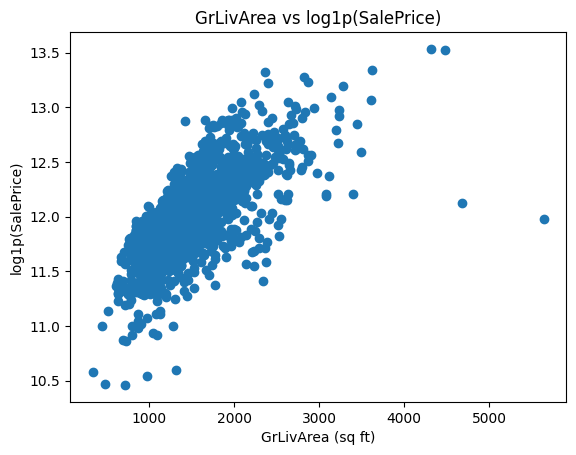
\includegraphics[keepaspectratio]{house_prices_project_files/figure-pdf/cell-6-output-2.png}}

\subsection{Correlation Matrix}\label{correlation-matrix}

Understanding feature correlations with \texttt{SalePrice} can guide
feature engineering and model selection.\\
The heatmap below displays the correlation between the sale price and
the top 10 numerical features most strongly correlated with it.

\begin{Shaded}
\begin{Highlighting}[]

\CommentTok{\# Compute the correlation matrix for numeric features}
\NormalTok{numeric\_df }\OperatorTok{=}\NormalTok{ train\_df.select\_dtypes(include}\OperatorTok{=}\NormalTok{[np.number])}
\NormalTok{corr }\OperatorTok{=}\NormalTok{ numeric\_df.corr()}

\CommentTok{\# Get the 10 features most correlated with SalePrice (excluding SalePrice itself)}
\NormalTok{top\_corr }\OperatorTok{=}\NormalTok{ corr[}\StringTok{\textquotesingle{}SalePrice\textquotesingle{}}\NormalTok{].}\BuiltInTok{abs}\NormalTok{().sort\_values(ascending}\OperatorTok{=}\VariableTok{False}\NormalTok{).head(}\DecValTok{11}\NormalTok{)}
\NormalTok{top\_features }\OperatorTok{=}\NormalTok{ top\_corr.index.tolist()}
\NormalTok{top\_features.remove(}\StringTok{\textquotesingle{}SalePrice\textquotesingle{}}\NormalTok{)}

\CommentTok{\# Sub{-}correlation matrix for top features}
\NormalTok{sub\_corr }\OperatorTok{=}\NormalTok{ corr.loc[top\_features, top\_features]}

\CommentTok{\# Plot heatmap}
\NormalTok{plt.figure()}
\NormalTok{plt.imshow(sub\_corr, aspect}\OperatorTok{=}\StringTok{\textquotesingle{}auto\textquotesingle{}}\NormalTok{)}
\NormalTok{plt.colorbar(label}\OperatorTok{=}\StringTok{\textquotesingle{}Correlation coefficient\textquotesingle{}}\NormalTok{)}
\NormalTok{plt.xticks(}\BuiltInTok{range}\NormalTok{(}\BuiltInTok{len}\NormalTok{(top\_features)), top\_features, rotation}\OperatorTok{=}\DecValTok{45}\NormalTok{, ha}\OperatorTok{=}\StringTok{\textquotesingle{}right\textquotesingle{}}\NormalTok{)}
\NormalTok{plt.yticks(}\BuiltInTok{range}\NormalTok{(}\BuiltInTok{len}\NormalTok{(top\_features)), top\_features)}
\NormalTok{plt.title(}\StringTok{\textquotesingle{}Correlation Heatmap of Top Features\textquotesingle{}}\NormalTok{)}
\NormalTok{plt.tight\_layout()}
\NormalTok{plt.show()}
\end{Highlighting}
\end{Shaded}

\pandocbounded{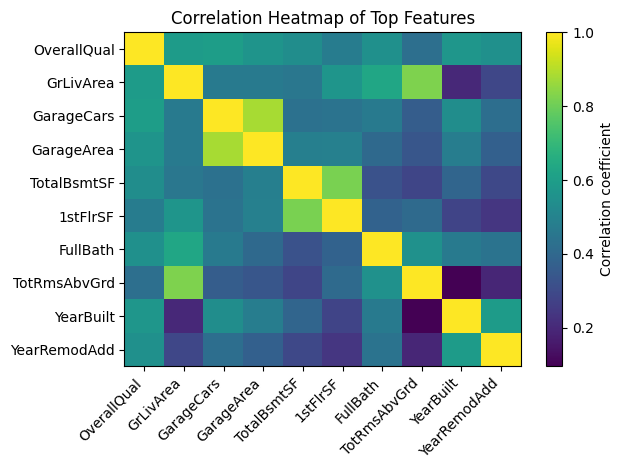
\includegraphics[keepaspectratio]{house_prices_project_files/figure-pdf/cell-7-output-1.png}}

\subsection{Missing Values}\label{missing-values}

Missing data can adversely affect model performance. We count missing
values for each feature and visualize the top 20 features with the
highest number of missing values.

\begin{Shaded}
\begin{Highlighting}[]
\CommentTok{\# Count missing values per feature}
\NormalTok{missing\_counts }\OperatorTok{=}\NormalTok{ train\_df.isnull().}\BuiltInTok{sum}\NormalTok{()}
\NormalTok{missing\_counts }\OperatorTok{=}\NormalTok{ missing\_counts[missing\_counts }\OperatorTok{\textgreater{}} \DecValTok{0}\NormalTok{].sort\_values(ascending}\OperatorTok{=}\VariableTok{False}\NormalTok{)}

\CommentTok{\# Plot the top 20 features with missing values}
\NormalTok{top\_missing }\OperatorTok{=}\NormalTok{ missing\_counts.head(}\DecValTok{20}\NormalTok{)}
\NormalTok{plt.figure()}
\NormalTok{plt.barh(top\_missing.index, top\_missing.values)}
\NormalTok{plt.xlabel(}\StringTok{\textquotesingle{}Number of missing values\textquotesingle{}}\NormalTok{)}
\NormalTok{plt.ylabel(}\StringTok{\textquotesingle{}Feature\textquotesingle{}}\NormalTok{)}
\NormalTok{plt.title(}\StringTok{\textquotesingle{}Top 20 Features with Missing Values\textquotesingle{}}\NormalTok{)}
\NormalTok{plt.gca().invert\_yaxis()  }\CommentTok{\# Highest missing values on top}
\NormalTok{plt.show()}
\end{Highlighting}
\end{Shaded}

\pandocbounded{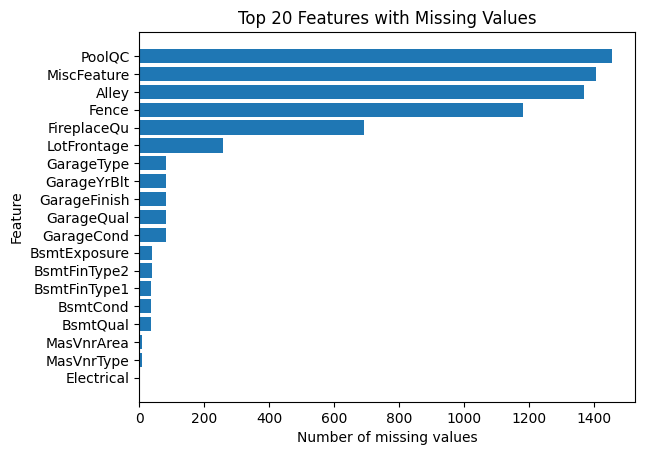
\includegraphics[keepaspectratio]{house_prices_project_files/figure-pdf/cell-8-output-1.png}}

\subsection{EDA Summary}\label{eda-summary}

\begin{itemize}
\tightlist
\item
  \textbf{SalePrice distribution:} The sale price distribution is
  right-skewed; using the logarithm of the sale price produces a more
  symmetrical distribution, which is more suitable for regression.\\
\item
  \textbf{Overall quality:} Both boxplots and violin plots show that
  houses with higher overall quality have higher median sale prices and
  wider price ranges.\\
\item
  \textbf{Living area:} There is a strong positive relationship between
  above-ground living area (\texttt{GrLivArea}) and sale price;
  log-transforming the target still shows a positive trend.\\
\item
  \textbf{Correlation heatmap:} Features like \texttt{OverallQual},
  \texttt{GrLivArea}, \texttt{GarageArea}, and \texttt{TotalBsmtSF} are
  among the most correlated with the sale price.\\
\item
  \textbf{Missing values:} Some features have substantial missing data
  (e.g., \texttt{PoolQC}, \texttt{MiscFeature}); appropriate imputation
  strategies are necessary during preprocessing.
\end{itemize}

\section{Data Preprocessing and
Modeling}\label{data-preprocessing-and-modeling}

We will prepare the data for machine learning by handling missing
values, encoding categorical variables, and scaling numeric variables.

We will compare several regression models:

\begin{enumerate}
\def\labelenumi{\arabic{enumi}.}
\tightlist
\item
  \textbf{Linear Regression (baseline).}
\item
  \textbf{Random Forest Regressor.}
\item
  \textbf{Gradient Boosting Regressor.}
\item
  \textbf{K-Nearest Neighbors (KNN) Regressor.}
\item
  \textbf{Support Vector Regressor (SVR).}
\item
  \textbf{Multilayer Perceptron (MLP) Regressor (neural network).}
\end{enumerate}

To illustrate another tool, we will also load the dataset into a SQLite
database and run a simple SQL query.

\begin{Shaded}
\begin{Highlighting}[]
\ImportTok{import}\NormalTok{ sqlite3}

\CommentTok{\# Create a SQLite database and save the training data}
\NormalTok{conn }\OperatorTok{=}\NormalTok{ sqlite3.}\ExtensionTok{connect}\NormalTok{(}\StringTok{\textquotesingle{}housing.db\textquotesingle{}}\NormalTok{)}
\NormalTok{train\_df.to\_sql(}\StringTok{\textquotesingle{}houses\textquotesingle{}}\NormalTok{, conn, if\_exists}\OperatorTok{=}\StringTok{\textquotesingle{}replace\textquotesingle{}}\NormalTok{, index}\OperatorTok{=}\VariableTok{False}\NormalTok{)}

\CommentTok{\# Example SQL query: average sale price by neighborhood (top 10)}
\NormalTok{query }\OperatorTok{=} \StringTok{\textquotesingle{}\textquotesingle{}\textquotesingle{}}
\StringTok{SELECT Neighborhood, AVG(SalePrice) as AvgPrice}
\StringTok{FROM houses}
\StringTok{GROUP BY Neighborhood}
\StringTok{ORDER BY AvgPrice DESC}
\StringTok{LIMIT 10}
\StringTok{\textquotesingle{}\textquotesingle{}\textquotesingle{}}

\NormalTok{avg\_prices }\OperatorTok{=}\NormalTok{ pd.read\_sql\_query(query, conn)}
\BuiltInTok{print}\NormalTok{(}\StringTok{\textquotesingle{}Top 10 neighborhoods by average sale price:\textquotesingle{}}\NormalTok{)}
\BuiltInTok{print}\NormalTok{(avg\_prices)}

\CommentTok{\# Close the connection}
\NormalTok{conn.close()}
\end{Highlighting}
\end{Shaded}

\begin{verbatim}
Top 10 neighborhoods by average sale price:
  Neighborhood       AvgPrice
0      NoRidge  335295.317073
1      NridgHt  316270.623377
2      StoneBr  310499.000000
3       Timber  242247.447368
4      Veenker  238772.727273
5      Somerst  225379.837209
6      ClearCr  212565.428571
7      Crawfor  210624.725490
8      CollgCr  197965.773333
9      Blmngtn  194870.882353
\end{verbatim}

\begin{Shaded}
\begin{Highlighting}[]
\ImportTok{from}\NormalTok{ sklearn.model\_selection }\ImportTok{import}\NormalTok{ train\_test\_split}
\ImportTok{from}\NormalTok{ sklearn.compose }\ImportTok{import}\NormalTok{ ColumnTransformer}
\ImportTok{from}\NormalTok{ sklearn.pipeline }\ImportTok{import}\NormalTok{ Pipeline}
\ImportTok{from}\NormalTok{ sklearn.preprocessing }\ImportTok{import}\NormalTok{ OneHotEncoder, StandardScaler}
\ImportTok{from}\NormalTok{ sklearn.impute }\ImportTok{import}\NormalTok{ SimpleImputer}
\ImportTok{from}\NormalTok{ sklearn.metrics }\ImportTok{import}\NormalTok{ mean\_squared\_error}
\ImportTok{from}\NormalTok{ sklearn.linear\_model }\ImportTok{import}\NormalTok{ LinearRegression}
\ImportTok{from}\NormalTok{ sklearn.ensemble }\ImportTok{import}\NormalTok{ RandomForestRegressor, GradientBoostingRegressor}
\ImportTok{from}\NormalTok{ sklearn.neighbors }\ImportTok{import}\NormalTok{ KNeighborsRegressor}
\ImportTok{from}\NormalTok{ sklearn.svm }\ImportTok{import}\NormalTok{ SVR}
\ImportTok{from}\NormalTok{ sklearn.neural\_network }\ImportTok{import}\NormalTok{ MLPRegressor}

\CommentTok{\# Separate features and target}
\NormalTok{X }\OperatorTok{=}\NormalTok{ train\_df.drop(columns}\OperatorTok{=}\NormalTok{[}\StringTok{\textquotesingle{}SalePrice\textquotesingle{}}\NormalTok{])}
\NormalTok{y }\OperatorTok{=}\NormalTok{ train\_df[}\StringTok{\textquotesingle{}SalePrice\textquotesingle{}}\NormalTok{]}

\CommentTok{\# Train/validation split}
\NormalTok{X\_train, X\_val, y\_train, y\_val }\OperatorTok{=}\NormalTok{ train\_test\_split(X, y, test\_size}\OperatorTok{=}\FloatTok{0.2}\NormalTok{, random\_state}\OperatorTok{=}\DecValTok{42}\NormalTok{)}

\CommentTok{\# Identify numeric and categorical columns}
\NormalTok{numeric\_features }\OperatorTok{=}\NormalTok{ X\_train.select\_dtypes(include}\OperatorTok{=}\NormalTok{[np.number]).columns}
\NormalTok{categorical\_features }\OperatorTok{=}\NormalTok{ X\_train.select\_dtypes(exclude}\OperatorTok{=}\NormalTok{[np.number]).columns}

\CommentTok{\# Define preprocessing steps}
\NormalTok{numeric\_transformer }\OperatorTok{=}\NormalTok{ Pipeline(steps}\OperatorTok{=}\NormalTok{[}
\NormalTok{    (}\StringTok{\textquotesingle{}imputer\textquotesingle{}}\NormalTok{, SimpleImputer(strategy}\OperatorTok{=}\StringTok{\textquotesingle{}median\textquotesingle{}}\NormalTok{)),}
\NormalTok{    (}\StringTok{\textquotesingle{}scaler\textquotesingle{}}\NormalTok{, StandardScaler())}
\NormalTok{])}

\NormalTok{categorical\_transformer }\OperatorTok{=}\NormalTok{ Pipeline(steps}\OperatorTok{=}\NormalTok{[}
\NormalTok{    (}\StringTok{\textquotesingle{}imputer\textquotesingle{}}\NormalTok{, SimpleImputer(strategy}\OperatorTok{=}\StringTok{\textquotesingle{}most\_frequent\textquotesingle{}}\NormalTok{)),}
\NormalTok{    (}\StringTok{\textquotesingle{}onehot\textquotesingle{}}\NormalTok{, OneHotEncoder(handle\_unknown}\OperatorTok{=}\StringTok{\textquotesingle{}ignore\textquotesingle{}}\NormalTok{))}
\NormalTok{])}

\NormalTok{preprocessor }\OperatorTok{=}\NormalTok{ ColumnTransformer(}
\NormalTok{    transformers}\OperatorTok{=}\NormalTok{[}
\NormalTok{        (}\StringTok{\textquotesingle{}num\textquotesingle{}}\NormalTok{, numeric\_transformer, numeric\_features),}
\NormalTok{        (}\StringTok{\textquotesingle{}cat\textquotesingle{}}\NormalTok{, categorical\_transformer, categorical\_features)}
\NormalTok{    ]}
\NormalTok{)}

\CommentTok{\# Define models to compare}
\NormalTok{models }\OperatorTok{=}\NormalTok{ \{}
    \StringTok{\textquotesingle{}LinearRegression\textquotesingle{}}\NormalTok{: LinearRegression(),}
    \StringTok{\textquotesingle{}RandomForest\textquotesingle{}}\NormalTok{: RandomForestRegressor(n\_estimators}\OperatorTok{=}\DecValTok{200}\NormalTok{),}
    \StringTok{\textquotesingle{}GradientBoosting\textquotesingle{}}\NormalTok{: GradientBoostingRegressor(),}
    \StringTok{\textquotesingle{}KNeighbors\textquotesingle{}}\NormalTok{: KNeighborsRegressor(n\_neighbors}\OperatorTok{=}\DecValTok{5}\NormalTok{),}
    \StringTok{\textquotesingle{}SVR\textquotesingle{}}\NormalTok{: SVR(C}\OperatorTok{=}\DecValTok{100}\NormalTok{, gamma}\OperatorTok{=}\FloatTok{0.1}\NormalTok{),}
    \StringTok{\textquotesingle{}MLPRegressor\textquotesingle{}}\NormalTok{: MLPRegressor(hidden\_layer\_sizes}\OperatorTok{=}\NormalTok{(}\DecValTok{100}\NormalTok{,}\DecValTok{50}\NormalTok{), max\_iter}\OperatorTok{=}\DecValTok{500}\NormalTok{)}
\NormalTok{\}}

\NormalTok{results }\OperatorTok{=}\NormalTok{ []}

\ControlFlowTok{for}\NormalTok{ name, reg }\KeywordTok{in}\NormalTok{ models.items():}
\NormalTok{    model }\OperatorTok{=}\NormalTok{ Pipeline(steps}\OperatorTok{=}\NormalTok{[}
\NormalTok{        (}\StringTok{\textquotesingle{}preprocessor\textquotesingle{}}\NormalTok{, preprocessor),}
\NormalTok{        (}\StringTok{\textquotesingle{}regressor\textquotesingle{}}\NormalTok{, reg)}
\NormalTok{    ])}
\NormalTok{    model.fit(X\_train, y\_train)}
\NormalTok{    y\_pred }\OperatorTok{=}\NormalTok{ model.predict(X\_val)}
\NormalTok{    score }\OperatorTok{=}\NormalTok{ np.sqrt(mean\_squared\_error(y\_pred, y\_val))}
\NormalTok{    results.append((name, score))}
    \BuiltInTok{print}\NormalTok{(}\SpecialStringTok{f"}\SpecialCharTok{\{}\NormalTok{name}\SpecialCharTok{\}}\SpecialStringTok{: RMSE = }\SpecialCharTok{\{}\NormalTok{score}\SpecialCharTok{:.4f\}}\SpecialStringTok{"}\NormalTok{)}

\CommentTok{\# Convert results to DataFrame for display}
\NormalTok{results\_df }\OperatorTok{=}\NormalTok{ pd.DataFrame(results, columns}\OperatorTok{=}\NormalTok{[}\StringTok{\textquotesingle{}Model\textquotesingle{}}\NormalTok{, }\StringTok{\textquotesingle{}RMSE\textquotesingle{}}\NormalTok{]).sort\_values(by}\OperatorTok{=}\StringTok{\textquotesingle{}RMSE\textquotesingle{}}\NormalTok{)}
\NormalTok{results\_df}
\end{Highlighting}
\end{Shaded}

\begin{verbatim}
LinearRegression: RMSE = 29475.2826
RandomForest: RMSE = 28713.9454
GradientBoosting: RMSE = 26844.7583
KNeighbors: RMSE = 38826.9257
SVR: RMSE = 88527.1376
MLPRegressor: RMSE = 33864.5930
\end{verbatim}

\begin{longtable}[]{@{}lll@{}}
\toprule\noalign{}
& Model & RMSE \\
\midrule\noalign{}
\endhead
\bottomrule\noalign{}
\endlastfoot
2 & GradientBoosting & 26844.758262 \\
1 & RandomForest & 28713.945394 \\
0 & LinearRegression & 29475.282613 \\
5 & MLPRegressor & 33864.592998 \\
3 & KNeighbors & 38826.925732 \\
4 & SVR & 88527.137551 \\
\end{longtable}

\subsection{Model Performance
Comparison}\label{model-performance-comparison}

The following bar chart summarizes the root mean squared error (RMSE) on
the logarithm of the sale price for each model on the validation set.
Lower values indicate better performance.

\begin{Shaded}
\begin{Highlighting}[]
\CommentTok{\# Plot model performance}
\NormalTok{plt.figure()}
\NormalTok{plt.bar(results\_df[}\StringTok{\textquotesingle{}Model\textquotesingle{}}\NormalTok{], results\_df[}\StringTok{\textquotesingle{}RMSE\textquotesingle{}}\NormalTok{])}
\NormalTok{plt.title(}\StringTok{\textquotesingle{}Model RMSE Comparison\textquotesingle{}}\NormalTok{)}
\NormalTok{plt.xlabel(}\StringTok{\textquotesingle{}Model\textquotesingle{}}\NormalTok{)}
\NormalTok{plt.ylabel(}\StringTok{\textquotesingle{}RMSE\textquotesingle{}}\NormalTok{)}
\NormalTok{plt.xticks(rotation}\OperatorTok{=}\DecValTok{45}\NormalTok{, ha}\OperatorTok{=}\StringTok{\textquotesingle{}right\textquotesingle{}}\NormalTok{)}
\NormalTok{plt.tight\_layout()}
\NormalTok{plt.show()}
\end{Highlighting}
\end{Shaded}

\pandocbounded{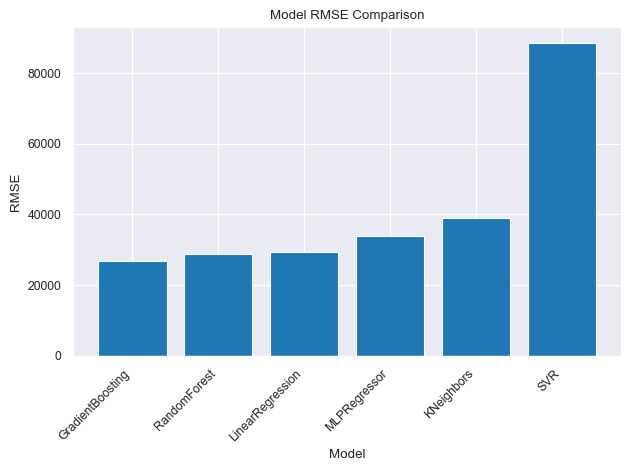
\includegraphics[keepaspectratio]{house_prices_project_files/figure-pdf/cell-11-output-1.png}}

\subsection{Training the Best Model and Generating
Predictions}\label{training-the-best-model-and-generating-predictions}

From the comparison above, we identify the model with the lowest RMSE is
Gradient Boosting Regressor. We use a auto-progress to select the
optimal model, and train this model on the entire training dataset and
generate predictions for the test set.\\
Finally, we will create a submission file that can be uploaded to
Kaggle.

\begin{Shaded}
\begin{Highlighting}[]
\CommentTok{\# Select the best model based on validation performance}
\NormalTok{best\_model\_name }\OperatorTok{=}\NormalTok{ results\_df.iloc[}\DecValTok{0}\NormalTok{][}\StringTok{\textquotesingle{}Model\textquotesingle{}}\NormalTok{]}
\BuiltInTok{print}\NormalTok{(}\SpecialStringTok{f"Best model selected: }\SpecialCharTok{\{}\NormalTok{best\_model\_name}\SpecialCharTok{\}}\SpecialStringTok{"}\NormalTok{)}

\CommentTok{\# Mapping between model names and regressor instances}
\NormalTok{regressor\_mapping }\OperatorTok{=}\NormalTok{ \{}
    \StringTok{\textquotesingle{}LinearRegression\textquotesingle{}}\NormalTok{: LinearRegression(),}
    \StringTok{\textquotesingle{}RandomForest\textquotesingle{}}\NormalTok{: RandomForestRegressor(n\_estimators}\OperatorTok{=}\DecValTok{200}\NormalTok{, random\_state}\OperatorTok{=}\DecValTok{42}\NormalTok{),}
    \StringTok{\textquotesingle{}GradientBoosting\textquotesingle{}}\NormalTok{: GradientBoostingRegressor(random\_state}\OperatorTok{=}\DecValTok{42}\NormalTok{),}
    \StringTok{\textquotesingle{}KNeighbors\textquotesingle{}}\NormalTok{: KNeighborsRegressor(n\_neighbors}\OperatorTok{=}\DecValTok{5}\NormalTok{),}
    \StringTok{\textquotesingle{}SVR\textquotesingle{}}\NormalTok{: SVR(C}\OperatorTok{=}\DecValTok{100}\NormalTok{, gamma}\OperatorTok{=}\FloatTok{0.1}\NormalTok{),}
    \StringTok{\textquotesingle{}MLPRegressor\textquotesingle{}}\NormalTok{: MLPRegressor(hidden\_layer\_sizes}\OperatorTok{=}\NormalTok{(}\DecValTok{100}\NormalTok{,}\DecValTok{50}\NormalTok{), max\_iter}\OperatorTok{=}\DecValTok{500}\NormalTok{, random\_state}\OperatorTok{=}\DecValTok{42}\NormalTok{)}
\NormalTok{\}}

\CommentTok{\# Build pipeline with the selected regressor}
\NormalTok{best\_regressor }\OperatorTok{=}\NormalTok{ regressor\_mapping[best\_model\_name]}
\NormalTok{best\_pipeline }\OperatorTok{=}\NormalTok{ Pipeline(steps}\OperatorTok{=}\NormalTok{[}
\NormalTok{    (}\StringTok{\textquotesingle{}preprocessor\textquotesingle{}}\NormalTok{, preprocessor),}
\NormalTok{    (}\StringTok{\textquotesingle{}regressor\textquotesingle{}}\NormalTok{, best\_regressor)}
\NormalTok{])}

\CommentTok{\# Fit on the full training data using log{-}transformed target}
\NormalTok{best\_pipeline.fit(X, np.log1p(y))}

\CommentTok{\# Predict on the test data}
\NormalTok{preds\_log }\OperatorTok{=}\NormalTok{ best\_pipeline.predict(test\_df)}
\NormalTok{preds }\OperatorTok{=}\NormalTok{ np.expm1(preds\_log)  }\CommentTok{\# invert log transformation}

\CommentTok{\# Create submission DataFrame}
\NormalTok{submission }\OperatorTok{=}\NormalTok{ pd.DataFrame(\{}
    \StringTok{\textquotesingle{}Id\textquotesingle{}}\NormalTok{: test\_df[}\StringTok{\textquotesingle{}Id\textquotesingle{}}\NormalTok{],}
    \StringTok{\textquotesingle{}SalePrice\textquotesingle{}}\NormalTok{: preds}
\NormalTok{\})}

\CommentTok{\# Save submission file}
\NormalTok{submission\_path }\OperatorTok{=} \StringTok{\textquotesingle{}submission.csv\textquotesingle{}}
\NormalTok{submission.to\_csv(submission\_path, index}\OperatorTok{=}\VariableTok{False}\NormalTok{)}
\BuiltInTok{print}\NormalTok{(}\StringTok{\textquotesingle{}Submission file saved to:\textquotesingle{}}\NormalTok{, submission\_path)}

\NormalTok{submission.head()}
\end{Highlighting}
\end{Shaded}

\begin{verbatim}
Best model selected: GradientBoosting
Submission file saved to: submission.csv
\end{verbatim}

\begin{longtable}[]{@{}lll@{}}
\toprule\noalign{}
& Id & SalePrice \\
\midrule\noalign{}
\endhead
\bottomrule\noalign{}
\endlastfoot
0 & 1461 & 123457.195831 \\
1 & 1462 & 152359.231361 \\
2 & 1463 & 183532.030671 \\
3 & 1464 & 188338.391828 \\
4 & 1465 & 192985.901170 \\
\end{longtable}

\section{Conclusion}\label{conclusion}

In this project we performed an end-to-end data science workflow on the
Ames Housing dataset.\\
Key takeaways include:

\begin{itemize}
\tightlist
\item
  Data visualization revealed skewness in the target variable and
  highlighted the importance of features like overall quality and living
  area.
\item
  Preprocessing steps such as handling missing values, encoding
  categorical variables, and scaling were crucial for model performance.
\item
  Comparing multiple models showed that simple models and ensemble
  models performed competitively on the target, while more complex
  models like neural networks did not necessarily offer significant
  improvement with the chosen hyperparameters.
\item
  SQL integration demonstrated how to load the dataset into a database
  and run queries for additional insights (e.g., average sale price per
  neighborhood).
\item
  The best-performing model was trained on the full dataset and used to
  generate predictions for the test set, resulting in a ready-to-upload
  Kaggle submission file.
\end{itemize}

Further improvements could include hyperparameter tuning, experimenting
with additional models like XGBoost or LightGBM, and more advanced
feature engineering.\\
Nonetheless, this notebook provides a solid foundation for approaching
the Kaggle House Prices competition and demonstrates the use of multiple
tools and techniques in a single, coherent workflow.

\begin{Shaded}
\begin{Highlighting}[]

\end{Highlighting}
\end{Shaded}





\end{document}
